\documentclass[10pt,twocolumn,letterpaper]{article}

\usepackage{cvpr}
\usepackage{times}
\usepackage{epsfig}
\usepackage{graphicx}
\usepackage{amsmath}
\usepackage{amssymb}

% Include other packages here, before hyperref.
\usepackage[pagebackref=true,breaklinks=true,letterpaper=true,colorlinks,bookmarks=false]{hyperref}

% Pages are numbered in submission mode, and unnumbered in camera-ready
\ifcvprfinal\pagestyle{empty}\fi
\begin{document}

%%%%%%%%% TITLE
\title{Genetic Snakes}
\cvprfinalcopy
\author{Konstantinos Katergaris\\
Arizona State University\\
1151 S Forest Ave, Tempe, AZ\\
{\tt\small kkaterga@asu.edu}}

%\thispagestyle{empty}

\maketitle
\begin{abstract}
This report implements an active contour model snakes using a genetic algorithm(GA). The genetic algorithm is used to find the best optimum parameters of the snake. Furthermore, snakes are used to detect object boundaries evolving iteratively. The genetic algorithm efficiently finds the optimal parameters that maximize the snake's performance on a specific image.
\end{abstract}
\section{Overview}
The snakes model is a active contour model  used for image contour detection. It minimizes the following energy function: \[ E_{\text{snake}} = E_{\text{int}} + E_{\text{image}} + E_{\text{ext}},\]. The snake’s shape and position adjust by minimizing this energy function to closely align with the target object’s contour in an image. More information can be found in the original paper \cite{4310076}.  To optimize the snake's parameters, a genetic algorithm (GA) was used. GAs are evolutionary optimizers inspired by natural selection. They work by initializing a population with random parameters, evaluating these parameters, and selecting the best ones. This process is repeated over multiple generations until the optimal parameters are found.

\section{Implementation}
The GA was implemented using the DEAP library, a framework for evolutionary algorithms in Python. The following parameters where set to be optimized. The GA works as follows: 
\begin{itemize}
    \item $\alpha$, $\beta$, and $\gamma$: control the snake's internal energy, determining its flexibility and smoothness.
    \item $w_{\text{edge}}$, $w_{\text{line}}$, $w_{\text{term}}$, $w_{\text{scale}}$: influence the snake’s interaction with image edges, lines, and other features.
    \item $\sigma$: controls the level of Gaussian smoothing applied to the image.
    \item Number of points: defines the number of points used in the snake
    \item Iterations: the number of iterations the snake evolves
\end{itemize}
The GA works as follows:

\begin{enumerate}
    \item \textbf{Initialization}: A population of individuals is created, each initialized as random snake parameter values. These initial values are generated within predefined ranges in the following Table ~\ref{tab:ga_params}
    \begin{table}[h!]
\centering
\begin{tabular}{|c|c|c|}
\hline
\textbf{Parameter}               & \textbf{Range}       \\ \hline
$\alpha$                      & [0.1, 0.2]           \\ \hline
$\beta$                         & [0.1, 0.5]           \\ \hline
$\gamma$                       & [0.01, 1.0]          \\ \hline
$w_{\text{edge}}$                & [0.5, 3.0]           \\ \hline
$w_{\text{line}}$         & [0.0, 1.0]           \\ \hline
$w_{\text{term}}$             & [0.0, 1.0]           \\ \hline
$w_{\text{scale}}$                & [0.0, 2.0]           \\ \hline
$\sigma$                     & [1.0, 5.0]           \\ \hline
\textit{num\_points}   & [20, 50]             \\ \hline
\textit{iterations}   & [100, 300]           \\ \hline
\end{tabular}
\caption{Ranges for parameters used in the Genetic Algorithm.}
\label{tab:ga_params}
\end{table}

    \item \textbf{Fitness Evaluation}: Each individual then attempts to fit the boundary of an object in an image with there given parameters. The fitness function evaluates how well the snake fits the object in the image by calculating the overlap between the snake contour and the target object. Additionally, external energy along the snake’s path is computed. 
    
    \item \textbf{Selection}: The GA then selects the best-performing individuals based on their fitness scores. This is done using a tournament method, where a portion of individuals are chosen to compete against each other and the one with the highest fitness score is selected.
    
  \item \textbf{Crossover and Mutation}: These selected individuals are recombined using crossover to create new offspring. Crossover is used to combine the parameters of two individuals. The genetic information, or parameters, of the parents is combined, and a new offspring is created, exchanging both of their best characteristics. A mutation is also applied to introduce variations, preventing early convergence and allowing the algorithm to perform for longer.

\item \textbf{Evolution}: Over successive generations, the population evolves, as the offspring replace their parents. The best individual in the final generation theoretically has the best parameters.
\end{enumerate}
The following paramaters where selected for the GA in ~\ref{tab:ga_algorithm_params}
\begin{table}[h!]
\centering
\begin{tabular}{|c|c|c|}
\hline
\textbf{Parameter}                                   & \textbf{Value}      \\ \hline
\textit{population\_size}         & 50                 \\ \hline
\textit{Number of generation}           & 20                 \\ \hline
\textit{ Crossover probability}                 & 0.7                \\ \hline
\textit{Mutation probability   }                                         & 0.2                \\ \hline
\textit{ Tournament size}                           & 3                  \\ \hline
\textit{Number of generations}                                       & 20                 \\ \hline
\textit{probability for mutation}              & 0.2                \\ \hline
\end{tabular}
\caption{Parameters of the Genetic Algorithm used in the optimization process.}
\label{tab:ga_algorithm_params}
\end{table}
\subsection{Experiments}
For the experiment a circle was generated. The following figure shows the end results of the GA with snakes

\begin{figure}[h!]
    \centering
    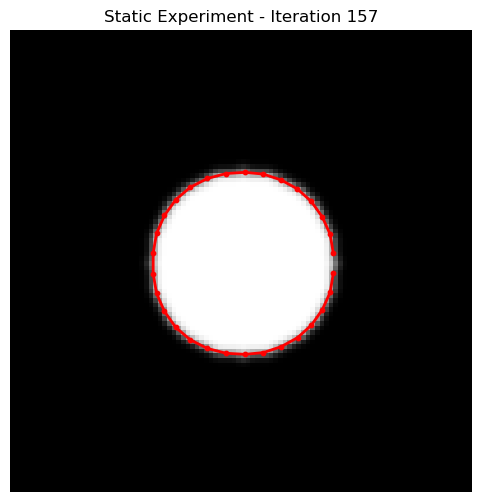
\includegraphics[width=1\linewidth]{47b4a0ee-e0b5-40a0-a248-65a246abff6a.png}
    \caption{Experiment where the snake fits on a generated circle}
    \label{fig:enter-label}
\end{figure}

Implementation can be found here : https://github.com/KostaKat/snakes.git


\section{Conclusion}
The genetic algorithm was effective at finding the best parameter for the snake to fit around the circle.

{\small
\bibliographystyle{ieee_fullname}
\bibliography{egbib}
}

\end{document}